\title{
	CSCI547 Machine Learning\\
	Homework 1\\
}
\author{
	Zachary Falkner\\
	Department of Computer Science\\
	University of Montana\\
}
\date{\today}
\documentclass[12pt]{article}

\usepackage{enumitem, listings, graphicx, xcolor, amsmath}

\lstset{language=Python,
	keywordstyle=\color{blue},
	basicstyle=\scriptsize\ttfamily,
	commentstyle=\ttfamily\itshape\color{gray},
	stringstyle=\ttfamily,
	showstringspaces=false,
	breaklines=true,
	frameround=ffff,
	frame=single,
	rulecolor=\color{black}
}

\begin{document}
	\maketitle
	
	\begin{flushleft}
		\section{Linear Regression}
		
		\subsection*{1A}
		$(X^T X + \gamma I_N) \vec{W} = X^TY$
		
		$\vec{w} = [w_0, w_1, w_2, w_3]$
		
		$X = $ \[
		\begin{bmatrix}
		1 & x_0 & x_0^2 & x_0^3 \\
		1 & x_1 & x_1^2 & x_1^3 \\
		... & ... & ... & ...\\
		1 & x_m & x_m^2 & x_m^3
		\end{bmatrix}
		\]
		
		$\mathcal{J} = \frac{1}{2} (\sum_{i=1}^{m} (y_i - w_0 - w_1 x_i - w_2 x_i^2 - w_3 x_i^3))^2$
		
		\vspace{0.5cm}
		
		$\frac{\partial \mathcal{J}}{\partial w_0} = - \sum_{i=1}^{m} (y_i - w_0 - w_1 x_i - w_2 x_i^2 - w_3 x_i^3)$
		
		$\frac{\partial \mathcal{J}}{\partial w_1} = - \sum_{i=1}^{m} (x_i (y_i - w_0 - w_1 x_i - w_2 x_i^2 - w_3 x_i^3)) + 2 \gamma w_1$
		
		$\frac{\partial \mathcal{J}}{\partial w_2} = - \sum_{i=1}^{m} (x_i^2 (y_i - w_0 - w_1 x_i - w_2 x_i^2 - w_3 x_i^3)) + 2 \gamma w_2$
		
		$\frac{\partial \mathcal{J}}{\partial w_3} = - \sum_{i=1}^{m} (x_i^3 (y_i - w_0 - w_1 x_i - w_2 x_i^2 - w_3 x_i^3)) + 2 \gamma w_3$
		
		\vspace{0.5cm}
		
		$\frac{\partial \mathcal{J}}{\partial w_0} = \sum_{i=1}^{m} (- y_i + w_0 + w_1 x_i + w_2 x_i^2 + w_3 x_i^3)$
		
		$\frac{\partial \mathcal{J}}{\partial w_1} = \sum_{i=1}^{m} (- y_i x_i + w_0 x_i - w_1 x_i^2 - w_2 x_i^3 - w_3 x_i^4) + 2 \gamma w_1$
		
		$\frac{\partial \mathcal{J}}{\partial w_2} = \sum_{i=1}^{m} (- y_i x_i^2 + w_0 x_i^2 + w_1 x_i^3 + w_2 x_i^4 + w_3 x_i^5) + 2 \gamma w_2$
		
		$\frac{\partial \mathcal{J}}{\partial w_3} = \sum_{i=1}^{m} (- y_i x_i^3 + w_0 x_i^3 + w_1 x_i^4 + w_2 x_i^5 + w_3 x_i^6) + 2 \gamma w_3$
		
				\vspace{0.5cm}
		
		$\frac{\partial \mathcal{J}}{\partial w_0} = 0 =\sum_{i=1}^{m} (- y_i + w_0 + w_1 x_i + w_2 x_i^2 + w_3 x_i^3)$
		
		$\frac{\partial \mathcal{J}}{\partial w_1} = 0 =\sum_{i=1}^{m} (- y_i x_i + w_0 x_i - w_1 x_i^2 - w_2 x_i^3 - w_3 x_i^4) + 2 \gamma w_1$
		
		$\frac{\partial \mathcal{J}}{\partial w_2} = 0 =\sum_{i=1}^{m} (- y_i x_i^2 + w_0 x_i^2 + w_1 x_i^3 + w_2 x_i^4 + w_3 x_i^5) + 2 \gamma w_2$
		
		$\frac{\partial \mathcal{J}}{\partial w_3} = 0 =\sum_{i=1}^{m} (- y_i x_i^3 + w_0 x_i^3 + w_1 x_i^4 + w_2 x_i^5 + w_3 x_i^6) + 2 \gamma w_3$
		
		\vspace{0.5cm}
		
		$\sum_{i=1}^{m} y_i = \sum_{i=1}^{m} (+ w_0 + w_1 x_i + w_2 x_i^2 + w_3 x_i^3)$
		
		$\sum_{i=1}^{m} y_i = \frac{\sum_{i=1}^{m} (w_0 x_i - w_1 x_i^2 - w_2 x_i^3 - w_3 x_i^4) + 2 \gamma w_1)}{x_i}$
		
		$\sum_{i=1}^{m} y_i = \frac{\sum_{i=1}^{m} (w_0 x_i^2 + w_1 x_i^3 + w_2 x_i^4 + w_3 x_i^5) + 2 \gamma w_2}{x_i^2}$
		
		$\sum_{i=1}^{m} y_i = \frac{\sum_{i=1}^{m} ( w_0 x_i^3 + w_1 x_i^4 + w_2 x_i^5 + w_3 x_i^6) + 2 \gamma w_3}{x_i^3}$
		
		\subsection*{1B}
\begin{lstlisting}
import pandas as pd
import numpy as np
import matplotlib as mpl
import matplotlib.pyplot as plt

#	degree - an arbitrary degree of polynomial
#	gamma - regularaztion strength (constant)
#	dataset - a pandas dataframe
#
def fit_with_l2(degree, gamma, dataset, test_set):
	#data and target from padas frame
	x = dataset[0].as_matrix().astype(float)
	y = dataset[1].as_matrix().astype(float)
	
	x_test = test_set[0].as_matrix().astype(float)
	y_test = test_set[1].as_matrix().astype(float)
	
	xhat = np.linspace(x.min(),x.max(), 200)
	Xhat = np.vander(xhat, N=degree + 1, increasing=True)
	x = 2*(dataset[0] - x.min())/(x.max()-x.min()) - 1  #this is x_tilde
	x_test = 2*(test_set[0] - x.min())/(x.max()-x.min()) - 1
	
	# Vandermond matrix (design matrix)
	X = np.vander(x,degree+1,increasing=True)
	
	# Identitity matrix for regularization
	Eye = np.eye(X.shape[1])
	#Eye hat, to not regularize bias
	Eye[0, 0] = 0
	
	# Solve for weight's set (params)  (training)
	w = np.linalg.solve(np.dot(X.T,X) + gamma*Eye,np.dot(X.T,y))
	
	yhat = np.dot(Xhat,w) # 250x2, 16x1
	
	X_test = np.vander(x_test, N=degree+1, increasing=True)
	
	avg_rmse = np.sqrt(np.sum((np.dot(X,w) - y)**2)/len(y))
	avg_rmse_test = np.sqrt(np.sum((np.dot(X_test, w) - y_test)**2)/len(y_test))
	
	plt.plot(x,y,'ro')
	plt.plot(xhat,yhat,'k-')
	plt.plot(x_test,test_set[1],'b*')
	plt.plot(x_test,y_test,'b^')
	plt.xlabel('Arbitrary Dataset Feature')
	plt.ylabel('Arbitrary Dataset Target')
	plt.show()

if __name__ == "__main__":
	dataset_file = "P1C_training.csv"
	testset_file = "P1C_test.csv"
	dataset = pd.read_csv(dataset_file, header=None)
	testset = pd.read_csv(testset_file, header=None)
	fit_with_l2(15, 1e-4, dataset, testset)
\end{lstlisting}
		
		\subsection*{1C}
		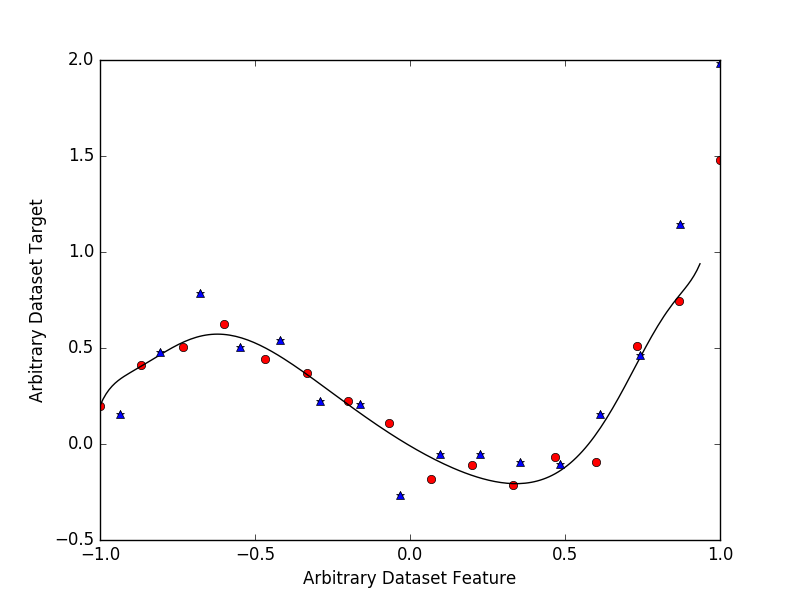
\includegraphics[scale=0.5]{HW1_1C.png}
		\label{fig:graph 1C}
		
		\subsection*{1D}
\begin{lstlisting}
import pandas as pd
import numpy as np
import matplotlib as mpl
import matplotlib.pyplot as plt

def fit_with_l2(degree, gamma, dataset, test_set):
	#data and target from padas frame
	x = dataset[0].as_matrix().astype(float)
	y = dataset[1].as_matrix().astype(float)
	
	x_test = test_set[0].as_matrix().astype(float)
	y_test = test_set[1].as_matrix().astype(float)
	
	xhat = np.linspace(x.min(),x.max(), 200)
	Xhat = np.vander(xhat, N=degree + 1, increasing=True)
	x = 2*(dataset[0] - x.min())/(x.max()-x.min()) - 1  #this is x_tilde
	x_test = 2*(test_set[0] - x.min())/(x.max()-x.min()) - 1
	
	# Vandermond matrix (design matrix)
	X = np.vander(x,degree+1,increasing=True)
	
	# Identitity matrix for regularization
	Eye = np.eye(X.shape[1])
	#Eye hat, to not regularize bias
	Eye[0, 0] = 0
	
	# Solve for weight's set (params)  (training)
	w = np.linalg.solve(np.dot(X.T,X) + gamma*Eye,np.dot(X.T,y))
	
	yhat = np.dot(Xhat,w) # 250x2, 16x1
	
	X_test = np.vander(x_test, N=degree+1, increasing=True)
	
	avg_rmse = np.sqrt(np.sum((np.dot(X,w) - y)**2)/len(y))
	avg_rmse_test = np.sqrt(np.sum((np.dot(X_test, w) - y_test)**2)/len(y_test))
	return avg_rmse, avg_rmse_test

if __name__ == "__main__":
	dataset_file = "P1C_training.csv"
	testset_file = "P1C_test.csv"
	dataset = pd.read_csv(dataset_file, header=None)
	testset = pd.read_csv(testset_file, header=None)
	
	degs = []
	rmses = []
	rmses_test = []
	
	for i in range(1, 16):
		avg_rmse, avg_rmse_test = fit_with_l2(i, 0, dataset, testset)
		degs.append(i)
		rmses.append(avg_rmse)
		rmses_test.append(avg_rmse_test)
	
	plt.plot(degs,rmses,'b-')
	plt.plot(degs, rmses_test, 'r-')
	plt.xlabel('Degree N')
	plt.ylabel('Average RMSE')
	plt.show()

\end{lstlisting}
		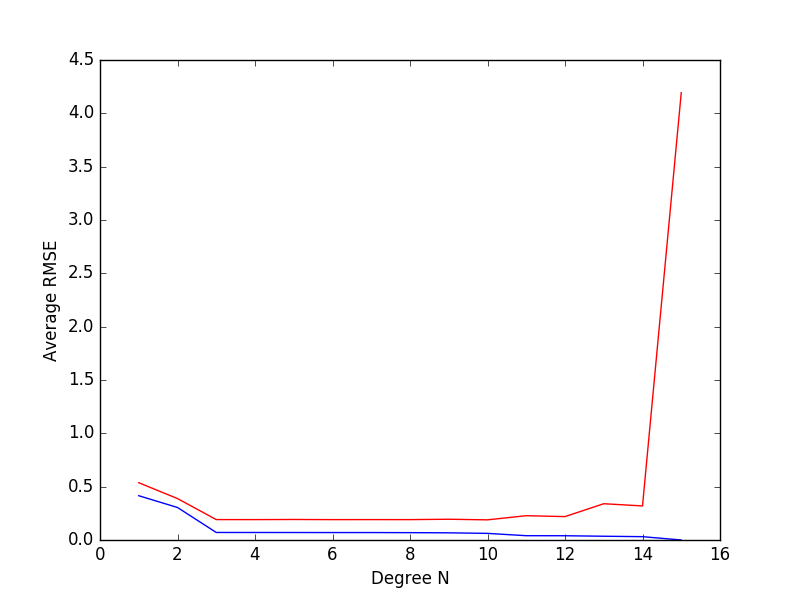
\includegraphics[scale=0.5]{HW1_1D.png}
		\label{fig:graph 1D}
		
		\subsection*{1E}
\begin{lstlisting}
import pandas as pd
import numpy as np
import matplotlib as mpl
import matplotlib.pyplot as plt

def fit_with_l2(degree, gamma, dataset, test_set):
	#data and target from padas frame
	x = dataset[0].as_matrix().astype(float)
	y = dataset[1].as_matrix().astype(float)
	
	x_test = test_set[0].as_matrix().astype(float)
	y_test = test_set[1].as_matrix().astype(float)
	
	xhat = np.linspace(x.min(),x.max(), 200)
	Xhat = np.vander(xhat, N=degree + 1, increasing=True)
	x = 2*(dataset[0] - x.min())/(x.max()-x.min()) - 1  #this is x_tilde
	x_test = 2*(test_set[0] - x.min())/(x.max()-x.min()) - 1
	
	# Vandermond matrix (design matrix)
	X = np.vander(x,degree+1,increasing=True)
	
	# Identitity matrix for regularization
	Eye = np.eye(X.shape[1])
	#Eye hat, to not regularize bias
	Eye[0, 0] = 0
	
	# Solve for weight's set (params)  (training)
	w = np.linalg.solve(np.dot(X.T,X) + gamma*Eye,np.dot(X.T,y))
	
	yhat = np.dot(Xhat,w) # 250x2, 16x1
	
	X_test = np.vander(x_test, N=degree+1, increasing=True)
	
	avg_rmse = np.sqrt(np.sum((np.dot(X,w) - y)**2)/len(y))
	avg_rmse_test = np.sqrt(np.sum((np.dot(X_test, w) - y_test)**2)/len(y_test))
	return avg_rmse, avg_rmse_test

if __name__ == "__main__":
	dataset_file = "P1C_training.csv"
	testset_file = "P1C_test.csv"
	dataset = pd.read_csv(dataset_file, header=None)
	testset = pd.read_csv(testset_file, header=None)
	
	rmses = []
	rmses_test = []
	
	gammas = np.logspace(-10, 3, 150)
	
	for i in gammas:
		avg_rmse, avg_rmse_test = fit_with_l2(15, i, dataset, testset)
		rmses.append(avg_rmse)
		rmses_test.append(avg_rmse_test)
	
	plt.semilogx(gammas,rmses,'b-')
	plt.semilogx(gammas, rmses_test, 'r-')
	plt.xlabel('Gamma')
	plt.ylabel('Average RMSE')
	plt.show()
\end{lstlisting}
		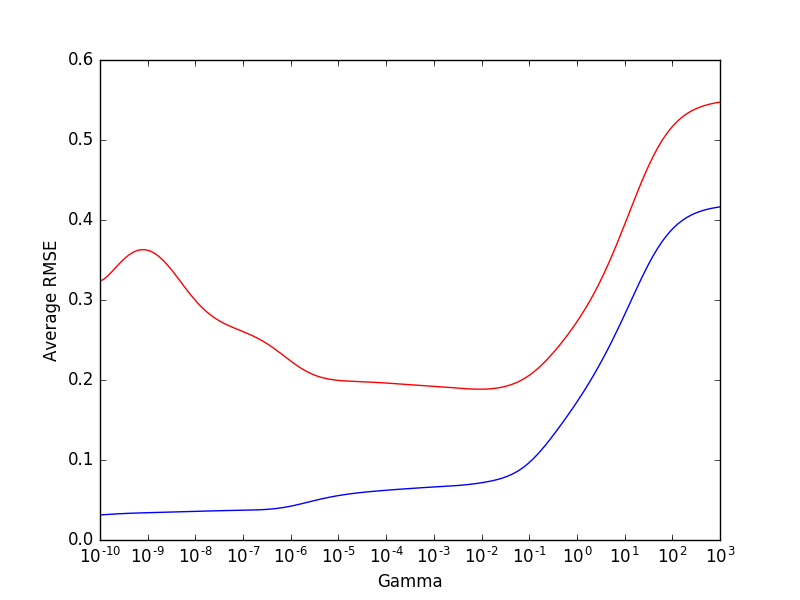
\includegraphics[scale=0.5]{HW1_1E.png}
		\label{fig:graph 1E}
		
		\subsection*{1F}
\begin{lstlisting}
import pandas as pd
import numpy as np
import matplotlib as mpl
import matplotlib.pyplot as plt
from sklearn import linear_model

def fit_with_l1(degree, gamma, dataset, test_set):
	#data and target from padas frame
	x = dataset[0].as_matrix().astype(float)
	y = dataset[1].as_matrix().astype(float)
	
	x_test = test_set[0].as_matrix().astype(float)
	y_test = test_set[1].as_matrix().astype(float)
	
	xhat = np.linspace(x.min(),x.max(), 200)
	Xhat = np.vander(xhat, N=degree + 1, increasing=True)
	x = 2*(dataset[0] - x.min())/(x.max()-x.min()) - 1  #this is x_tilde
	x_test = 2*(test_set[0] - x.min())/(x.max()-x.min()) - 1
	
	# Vandermond matrix (design matrix)
	X = np.vander(x,degree+1,increasing=True)
	
	# Identitity matrix for regularization
	Eye = np.eye(X.shape[1])
	#Eye hat, to not regularize bias
	Eye[0, 0] = 0
	
	# Solve for weight's set (params)  (training)
	w = np.linalg.solve(np.dot(X.T,X) + gamma*Eye,np.dot(X.T,y))
	
	yhat = np.dot(Xhat,w) # 250x2, 16x1
	
	X_test = np.vander(x_test, N=degree+1, increasing=True)
	
	lasso = linear_model.Lasso(alpha=gamma, max_iter=10000000)
	lasso.fit(X, y)
	
	avg_rmse = np.sqrt(np.sum((np.dot(X,w) - y)**2)/len(y))
	avg_rmse_test = np.sqrt(np.sum((np.dot(X_test, w) - y_test)**2)/len(y_test))
	return avg_rmse, avg_rmse_test


if __name__ == "__main__":
	dataset_file = "P1C_training.csv"
	testset_file = "P1C_test.csv"
	dataset = pd.read_csv(dataset_file, header=None)
	testset = pd.read_csv(testset_file, header=None)
	
	rmses = []
	rmses_test = []
	
	gammas = np.logspace(-10, 3, 40)
	
	for i in gammas:
		print("running lasso {}".format(i))
		avg_rmse, avg_rmse_test = fit_with_l1(15, i, dataset, testset)
		rmses.append(avg_rmse)
		rmses_test.append(avg_rmse_test)
	
	plt.semilogx(gammas,rmses,'b-')
	plt.semilogx(gammas, rmses_test, 'r-')
	plt.xlabel('Gamma')
	plt.ylabel('Average RMSE')
	plt.show()
\end{lstlisting}
		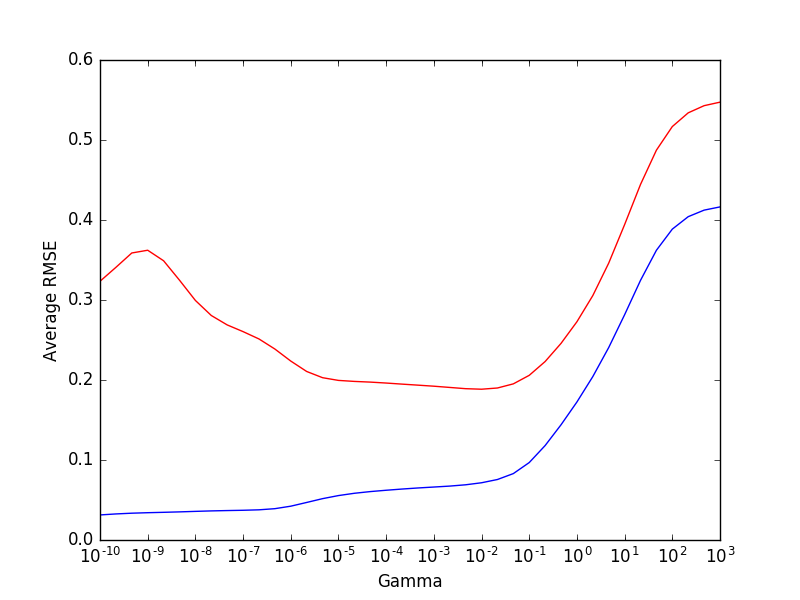
\includegraphics[scale=0.5]{HW1_1F.png}
		\label{fig:graph 1F}
		
		\vspace{0.5cm}
		The plots look nearly identical to me with the exception that 1E is smoother because i used less points in 1F (Lasso takes a long time to run with small alphas)
		
		\subsection*{1G*}
\begin{lstlisting}
import pandas as pd
import numpy as np
import matplotlib as mpl
import matplotlib.pyplot as plt

def fit_with_l2(degree, gamma, dataset, test_set):
	#data and target from padas frame
	x = dataset[0].as_matrix().astype(float)
	y = dataset[1].as_matrix().astype(float)
	
	x_test = test_set[0].as_matrix().astype(float)
	y_test = test_set[1].as_matrix().astype(float)
	
	xhat = np.linspace(x.min(),x.max(), 200)
	Xhat = np.vander(xhat, N=degree + 1, increasing=True)
	x = 2*(dataset[0] - x.min())/(x.max()-x.min()) - 1  #this is x_tilde
	x_test = 2*(test_set[0] - test_set[0].min())/(test_set[0].max()-test_set[0].min()) - 1
	
	# Vandermond matrix (design matrix)
	X = np.polynomial.legendre.legvander(x,degree)
	
	# Identitity matrix for regularization
	Eye = np.eye(X.shape[1])
	#Eye hat, to not regularize bias
	Eye[0, 0] = 0
	
	# Solve for weight's set (params)  (training)
	w = np.linalg.solve(np.dot(X.T,X) + gamma*Eye,np.dot(X.T,y))
	
	yhat = np.dot(Xhat,w) # 250x2, 16x1
	
	X_test = np.polynomial.legendre.legvander(x_test, degree)
	
	avg_rmse = np.sqrt(np.sum((np.dot(X,w) - y)**2)/len(y))
	avg_rmse_test = np.sqrt(np.sum((np.dot(X_test, w) - y_test)**2)/len(y_test))
	return avg_rmse, avg_rmse_test

if __name__ == "__main__":
	dataset_file = "P1C_training.csv"
	testset_file = "P1C_test.csv"
	dataset = pd.read_csv(dataset_file, header=None)
	testset = pd.read_csv(testset_file, header=None)
	
	degs = []
	rmses = []
	rmses_test = []
	
	for i in range(1, 21):
		avg_rmse, avg_rmse_test = fit_with_l2(i, 0, dataset, testset)
		degs.append(i)
		rmses.append(avg_rmse)
		rmses_test.append(avg_rmse_test)
	
	plt.plot(degs,rmses,'b-')
	plt.plot(degs, rmses_test, 'r-')
	plt.xlabel('Degree N')
	plt.ylabel('Average RMSE')
	plt.show()

\end{lstlisting}
		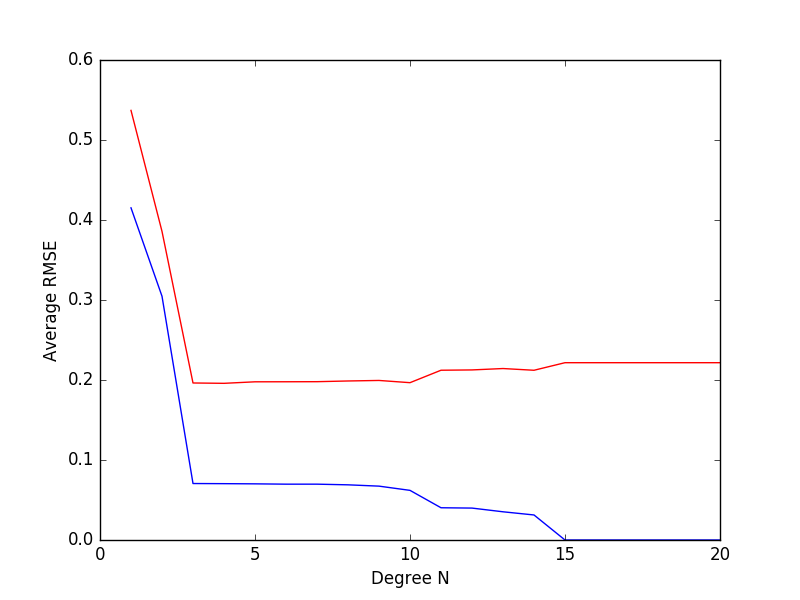
\includegraphics[scale=0.5]{HW1_1G.png}
		\label{fig:graph 1G}
		\section*{Probability and Bayes Theorem}
		
		\subsection*{2A Bayesian Inference}
		$P(D) = 10^{-4}$\\
		$P(\neg D) = 1 - 10^{-4}$\\
		$P(T|D) = 0.99$\\
		$P(T) = P(D)P(T|D) + P(\neg D) P(\neg T|D)$\\
		$P(D|T) = \frac{P(T|D) P(D)}{P(T)}$\\
		$P(D|T) = \frac{P(T|D) P(D)}{P(T)}$\\
		
		$P(D|T) = \frac{P(T|D) P(D)}{P(D)P(T|D) + P(\neg D) P(\neg T|D)}$\\
		
		$P(D|T) = \frac{0.99 * 10^{-4}}{10^{-4} * 0.99 + (1 - 10^{-4}) * 0.01}$\\
		$P(D|T) = 0.0098039$\\
		
		$P(T_N|D) = 0.99999$\\
		$P(D|T_N) = \frac{0.99999 * 10^{-4}}{10^{-4} * 0.99999 + (1 - 10^{-4}) * 0.00001}$\\
		$P(D|T) = 0.9090983$\\
		
		\subsection*{2B Bayesian Linear Regression}
		
		\subsection*{2C* Updating Bayesian Linear Regression}
		
		\section*{Naive Bayes}
		
		\subsection*{3A}
		We do not need to compute the denomenator in the classification rule for Naive Bayes because we are assuming  the data is independent and identically distributed. That is, it is a normal distribution with no dependence between features.
		
		\subsection*{3B}
\begin{lstlisting}
import pandas as pd
import numpy as np
import matplotlib as mpl
import matplotlib.pyplot as plt

from sklearn.datasets import load_digits
from sklearn.model_selection import train_test_split
from sklearn.metrics import confusion_matrix


if __name__ == "__main__":
	digits = load_digits()
	data = np.round(digits['data']/16.0)
	
	X = data    # n x m matrix of features 
	y = digits.target  # n vector of classes
	X,X_test,y,y_test = train_test_split(X,y,test_size=0.33,random_state=42) # Split into 33% test and 67% training sets 
	
	classes = np.linspace(0,9,10) 
	
	m = X.shape[0]  # Number of data instances
	m_test = X_test.shape[0] # Number of test data instances
	N = 10           # Number of classes
	n = X.shape[1]  # Number of features
	
	mu_array = np.zeros((n,N))
	sigma2_array = np.zeros((n,N))
	prior_array = np.zeros((N))
	
	#Learning phase
	for k in range(N):    #Loop over each class label
		C_k = classes[k]
		prior = sum(y==C_k)/float(y.shape[0])                           # Count the number of data where the label is C_k
		mu = np.sum(X[y==C_k],axis=0)/len(X[y==C_k])                    # Take the mean of those features where the corresponding label is C_k
		mu_array[:,k] = mu                                              # Store in the arrays we created above
		prior_array[k] = prior
	
	class_probabilities = np.zeros((m,N))  # The probabilities for 
	
	for i,x in enumerate(X):  # Loop over the training data instances
		for k in range(N):    # Loop over the classes
			prior = prior_array[k]
			mu = mu_array[:,k]
			# likelihood = np.prod(np.exp(-(x-mu)**2/(2*sigma2))) #change me
			likelihood = np.prod(np.power(mu, x) * np.power((1-mu), 1-x) )
			posterior_k = prior*likelihood
			class_probabilities[i,k] = posterior_k
	
	class_probabilities /= np.sum(class_probabilities,axis=1,keepdims=True)
	
	y_pred_train = np.argmax(class_probabilities,axis=1)
	
	cm_train = confusion_matrix(y,y_pred_train)
	print(cm_train)
	print("training accuracy:", 1 - sum(abs(y!=y_pred_train))/float(m))
	
	
	# Test set predictions
	class_probabilities = np.zeros((m_test,N))
	
	for i,x in enumerate(X_test):
		for k in range(N):
			prior = prior_array[k]
			mu = mu_array[:,k]
			sigma2 = sigma2_array[:,k]
			likelihood = np.prod(np.power(mu, x) * np.power((1-mu), 1-x) )
			posterior_k = prior*likelihood
			class_probabilities[i,k] = posterior_k
	
	class_probabilities /= class_probabilities.sum(axis=1,keepdims=True)
	y_pred_test = np.argmax(class_probabilities,axis=1)
	
	cm_test = confusion_matrix(y_test,y_pred_test)
	print(cm_test)
	print("test accuracy:", 1 - sum(abs(y_test-y_pred_test))/float(m_test))

\end{lstlisting}
\vspace{0.5cm}
training confusion matrix:
\[
\begin{bmatrix}
119  &0    &0    &0    &1    &2    &0    &0    &0    &1\\
0    &108  &4    &0    &0    &1    &1    &0    &7    &6\\
1    &2    &116  &1    &0    &0    &0    &0    &2    &3\\
0    &2    &1    &111  &0    &2    &0    &6    &2    &3\\
0    &1    &0    &0    &108  &0    &1    &4    &3    &0\\
0    &0    &1    &2    &1    &99   &0    &0    &0    &6\\
0    &3    &0    &0    &1    &0    &119  &0    &1    &0\\
0    &0    &1    &0    &0    &0    &0    &115  &1    &0\\
0    &11   &3    &0    &0    &3    &0    &2    &101  &2\\
0    &0    &0    &2    &0    &2    &0    &3    &2    &103\\
\end{bmatrix}
\]
training accuracy: 0.913549459684\\


\vspace{1cm}
testing confusion matrix:
\[
\begin{bmatrix}
52  &0   &0   &0   &2   &1   &0   &0   &0   &0\\
0   &37  &5   &0   &1   &0   &0   &0   &7   &5\\
0   &4   &46  &0   &0   &0   &0   &0   &2   &0\\
0   &0   &2   &45  &0   &0   &0   &1   &3   &5\\
0   &0   &0   &0   &63  &0   &0   &1   &0   &0\\
2   &0   &0   &0   &1   &60  &0   &0   &0   &10\\
0   &0   &0   &0   &0   &1   &55  &0   &1   &0\\
1   &0   &1   &0   &0   &1   &0   &58  &0   &1\\
0   &2   &2   &1   &0   &1   &0   &0   &45  &1\\
0   &0   &0   &4   &0   &1   &0   &4   &2  &57\\
\end{bmatrix}
\]
test accuracy: 0.872053872054\\
		
	\end{flushleft}
\end{document}